\documentclass{article}
\usepackage{graphicx}
\usepackage{hyperref}
\usepackage{listings}
\usepackage{xcolor}
\usepackage{tikzsymbols}
\usepackage{float}

\lstset{
    basicstyle=\ttfamily,
    backgroundcolor=\color{gray!30},
}

\begin{document}

\graphicspath{ {./Images/} }
\tableofcontents

\section{Introduction}
Words

\section{Domain Controller}

\subsection{Network}
Control Panel $\rightarrow$ Network and Sharing Center $\rightarrow$
Change Adapter Settings $\rightarrow$ Click "Internet Protocol Version 4 (TCP/IPv4)

\begin{figure}[]
        \centering
        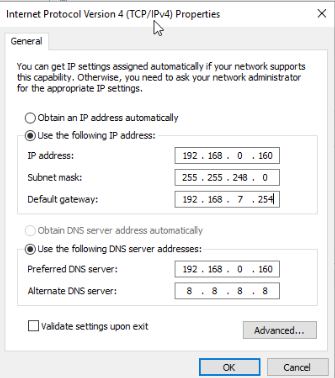
\includegraphics[width=1\textwidth]{SampleDCIPv4.png}
        \caption{Example IPv4 Settings}
        \label{fig:IPv4Settings}
\end{figure}

There are two things happening: setting a static IP and setting the DNS server

\subsubsection{Setting a Static IP}
For an image, see Figure~\ref{fig:IPv4Settings}

\noindent Look up how IP addresses work if you need to.

You can set the static IP to any IP not currently in use.
Maybe you can kick machines without a static IP off of their IP, but that is probably not advised.
Once you have picked your IP, put it in the \textbf{IP Address} field.
I am not sure how to determine the subnet mask manually, but I run \textbf{ipconfig} in powershell
and use the subnet mask it gives.
To determine the default gateway, you can run \textbf{ipconfig} or \textbf{route print}.
Bing was telling me to find it by running \textbf{ip route show} on the Proxmox console.


\subsubsection{Setting the DNS Servers}
For an image, see Figure~\ref{fig:IPv4Settings}

This step is less complicated than the last step. However, you can Red-Team yourself (I speak from experience...), so be careful.
On the Domain Controller, the first DNS server should be itself (the same as the machine's static IP). The second should be an actual internet DNS server.
In this case 8.8.8.8 is Google's DNS Server.

\end{document}